\section{Design decisions}

\subsection{Database} \label{db_disc}
We use MongoDB for our database. We chose to use this database as it is easy to implement and easy to use. We have
a MongoDB database with 1 collection, Bikes. The Bikes collection stores all bike locations and their availability. There should be a second database collection, Users, for storing the name, passwords and a list of rented bikes. Due to lack of time, we weren't able to implement this correctly.

    \begin{figure}[H]
		\centering
		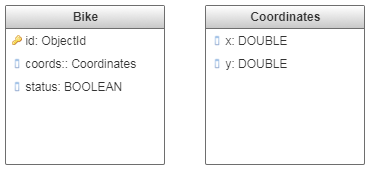
\includegraphics[width=0.3\textwidth]{images/db-structure.png}
		\caption{Overview of the database}
		\label{database}
	\end{figure}


In the docker swarm mode, the Mongo replica set is used to enable sharing of the data between the instances of MongoDB on different hosts. Replica sets provide redundancy and increase the availability of the data. All write operations are performed to the primary node and then replicated to the secondary nodes, as shown in \autoref{repl}.

    \begin{figure}[H]
		\centering
		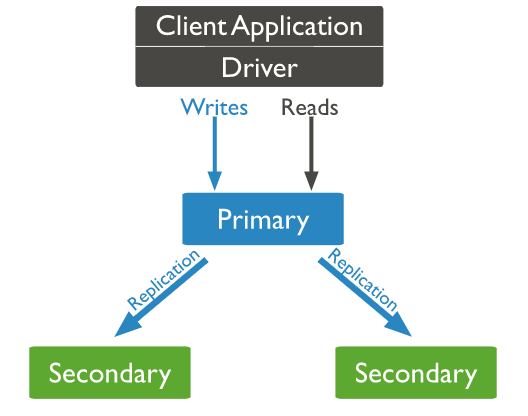
\includegraphics[width=0.7\textwidth]{images/replication.png}
		\caption{Replica sets in MongoDB}
		\label{repl}
	\end{figure}


As opposed to the other services that are deployed in the docker swarm mode, MongoDB needs some additional configuration. Docker cannot take care of initializing the replica set and making sure that the data is correctly replicated among different nodes. This means that we have to manage the replica set by ourselves. If the replica set is configured manually there is a high risk that if one of the MongoDB instances goes down and appears again, its IP address will be different and the replica set will need to be reconfigured (the new IP address of the node should be added and the old one removed). This may cause the read and write operations to fail, which is not what we want. So we have found a way to deal with this problem. We have a separate container (called controller) that maintains the replica set up and running and updates the configuration whenever necessary.  This container does not need replication and is deployed only once on the manager node. So the backend, when deployed in the swarm mode, looks as it is represented in \autoref{backend}.

    \begin{figure}[H]
		\centering
		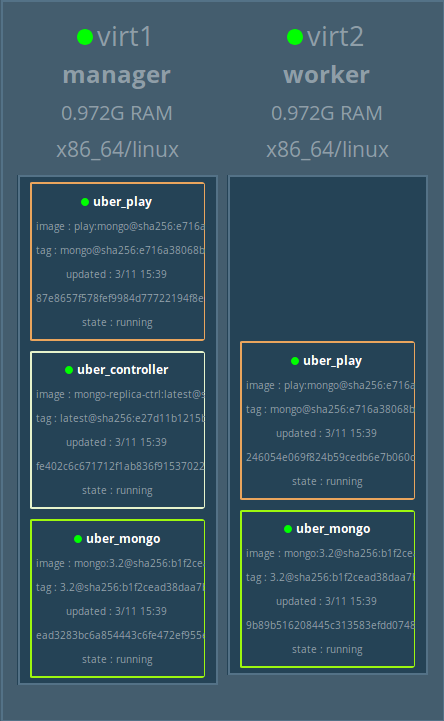
\includegraphics[width=0.7\textwidth]{images/backend.png}
		\caption{MongoDB replication in docker swarm mode}
		\label{repl}
	\end{figure}


\subsection{Webserver}
We chose Play as the framework for back-end development of our application mostly because it supports asynchronous I/O. There were two main causes for choosing Scala: the first is the possibility to learn a new programming language and the second is professor's incentive to use Scala for back-end development. In the end we succeeded in building a working back-end. We benefited from online completed projects we found on the internet as it aided our understanding and development of the final product. During the development we had difficulties connecting our database with Play as well as using WebSockets for live data streaming.

\subsection{Client}
Angular is a framework for building Web single-page applications and Bootstrap is an easy to use front-end web framework for designing web applications. These are the main reasons why we chose to use these frameworks. Other advantage of using Angular is its highly readable and comprehensive code. It was an important factor because we wanted something that will take as little time to learn as possible. We created the project using Angular Cli and used components to create the navigation bar, map component, and two (login and registration) forms (unfortunately not seen in the final layout). Even if it is not linked to framework itself, we found useful the large community of developers using Angular as online answers helped us solve most encountered problems.

\begin{figure}[H]
		\centering
		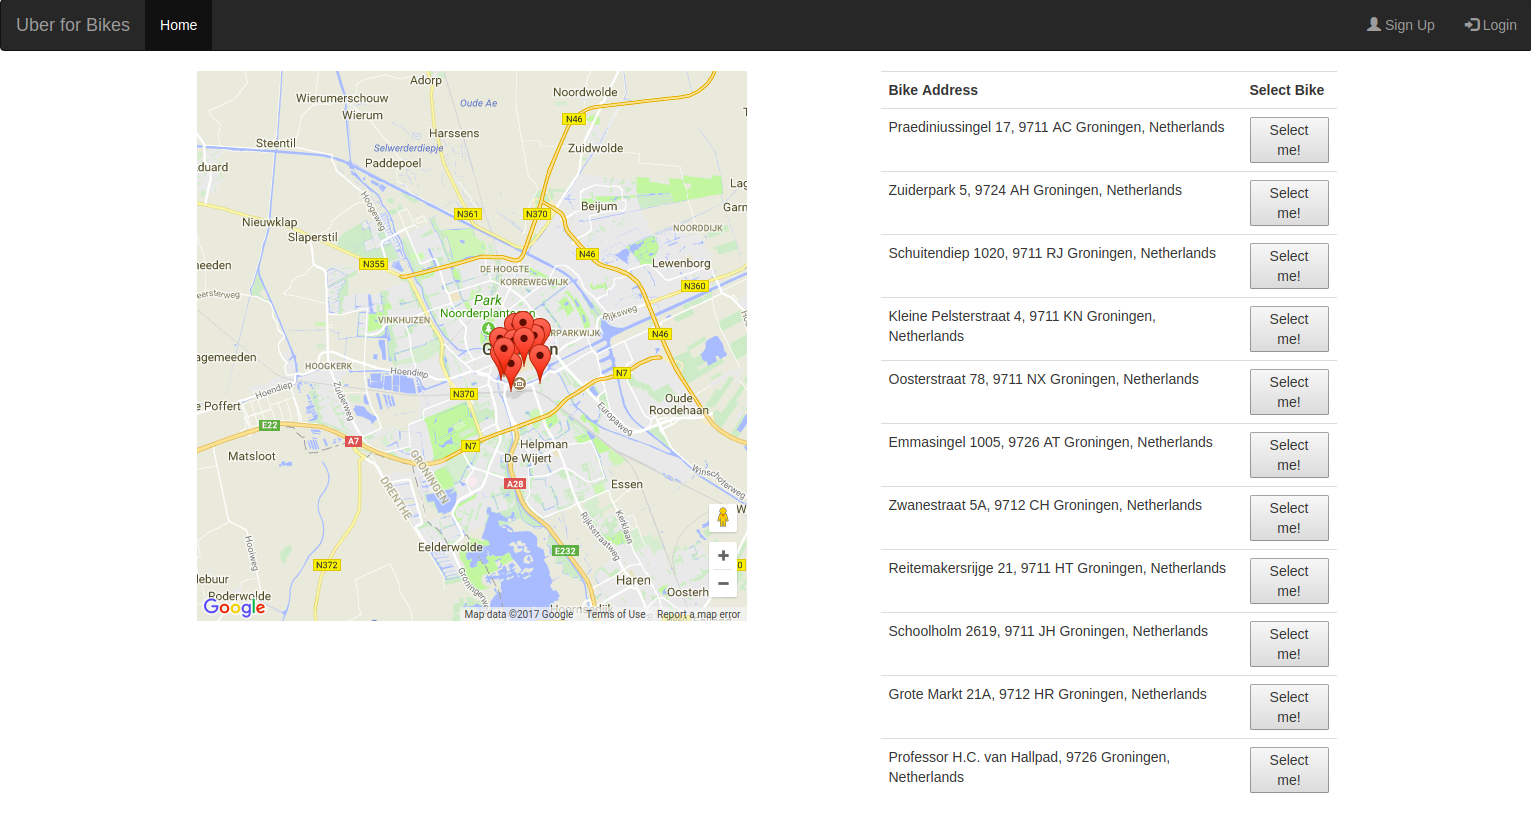
\includegraphics[width=0.9\textwidth]{images/screenshot.png}
		\caption{Application layout}
		\label{front-end}
	\end{figure}